\documentclass[11pt]{article}

\usepackage[a4paper,margin=1in]{geometry}
\usepackage{amsmath,amssymb,amsthm}
\usepackage{bm}
\usepackage{booktabs}
\usepackage{tikz}
\usepackage[hidelinks]{hyperref}
\usepackage{enumitem}

\newtheorem{definition}{Definition}
\newtheorem{proposition}{Proposition}
\newtheorem{theorem}{Theorem}
\newtheorem{remark}{Remark}

\newcommand{\R}{\mathbb{R}}
\newcommand{\Ein}{\mathcal{E}_{\mathrm{in}}}
\newcommand{\zbf}{\bm{\zeta}}
\newcommand{\abf}{\bar{\bm{a}}}
\newcommand{\Gbf}{\bm{G}}
\newcommand{\ubf}{\bm{u}}
\newcommand{\pbf}{\bm{p}}
\newcommand{\inner}[2]{\langle #1,\, #2\rangle}

\title{\textbf{Hamilton--Jacobi--Bellman Reachability for a\\
Twin--Thruster Surface Vessel Pursuing an\\
Artificial--Potential--Field Evader}\\[4pt]
\large Updated Methodology: Control Model, Value Function, and Viscosity Solution}
\author{}
\date{\today}

\begin{document}
\maketitle

\begin{abstract}
This document states the corrected mathematical formulation for the guaranteed-capture
problem in which a single \emph{pursuer} twin-thruster autonomous surface vessel, governed by
full three-degree-of-freedom Fossen dynamics, must capture an \emph{evader} vessel that executes
a fixed repulsive artificial-potential-field feedback law. Because the evader control is a known
function of the state, the two-player differential game collapses to a single-player optimal
control problem, and the governing equation is a Hamilton--Jacobi--Bellman (HJB) variational
inequality rather than a Hamilton--Jacobi--Isaacs (HJI) equation. Three corrections relative to
the previous draft are incorporated: (i) the actuator constraint is modelled as the
\emph{largest ellipse inscribed} in the true (offset) thrust polytope, yielding a conservative,
smooth, closed-form Hamiltonian with a previously-missing affine bias term; (ii) the artificial
viscosity (Laplacian) term is removed from the \emph{definition} of the value function and, if
used at all, appears only as an annealed regulariser in the training loss; and (iii) the value
function is defined directly as an optimal-control quantity and shown, through the dynamic
programming principle, to be the unique viscosity solution of the first-order variational
inequality. A physics-informed neural network solution method and a verification protocol are
specified.
\end{abstract}

\tableofcontents

\section{Problem setting and why the equation is HJB, not HJI}

Two identical twin-thruster autonomous surface vessels operate in the horizontal plane: a
\emph{pursuer} (subscript $i$) and an \emph{evader} (subscript $e$). The pursuer seeks to reduce
the inter-vessel separation below a capture radius $\rho>0$; the evader seeks to avoid this. The
single modelling assumption that distinguishes this problem from a two-player differential game is
that the evader does not optimise: its thruster commands are set by a fixed, known repulsive
artificial-potential-field (APF) feedback law. Consequently the only decision-maker is the
pursuer, and the problem is a single-player optimal control problem whose value function obeys a
Hamilton--Jacobi--Bellman (HJB) equation.

\begin{remark}[HJB versus HJI]
The difference between the two equations is only the Hamiltonian. A Hamilton--Jacobi--Isaacs (HJI)
game Hamiltonian contains a nested optimisation, $\min_{u_i}\max_{u_e}\inner{\pbf}{f}$; the HJB
Hamiltonian contains a single optimisation, $\min_{u_i}\inner{\pbf}{f}$, because the evader input
$u_e$ has been fixed to the APF law and absorbed into the drift. Everything concerning the
\emph{viscosity solution} is identical in the two cases: the notion was developed originally for
single-player HJB (Bellman) equations, and the non-smoothness of the value function is a property
of the first-order nonlinear equation, not of the presence of an adversary.
\end{remark}

\begin{remark}[Scope of the guarantee]
The backward reachable tube computed here certifies capturability against an evader executing the
specified APF policy. It is not a worst-case (game-theoretic) guarantee. This is a deliberate,
clearly-scoped modelling choice that trades game-theoretic coverage for a simpler HJB problem.
\end{remark}

\section{Vessel dynamics and the control-affine reduced system}

Each vessel obeys the standard three-degree-of-freedom manoeuvring (Fossen) model
$\bm{M}\dot{\bm{\nu}}+\bm{C}(\bm{\nu})\bm{\nu}+\bm{D}(\bm{\nu})\bm{\nu}=\bm{\tau}$, with body-frame
velocity $\bm{\nu}=(u,v,r)^\top$ (surge, sway, yaw rate) and generalised force
$\bm{\tau}=(\tau_u,0,\tau_r)^\top$; the sway force is identically zero because two fixed parallel
thrusters produce only surge force and yaw moment. Under port--starboard symmetry the mass matrix
is diagonal, $\bm{M}=\mathrm{diag}(M_{11},M_{22},M_{33})$.

Working in the pursuer body frame, define the nine-dimensional relative state
\begin{equation}
\zbf=\big(X,\;Y,\;\psi_{\mathrm{rel}},\;u_e,\;v_e,\;u_i,\;v_i,\;r_e,\;r_i\big)^\top\in\R^9 ,
\end{equation}
where $(X,Y)$ is the evader position relative to the pursuer, $\psi_{\mathrm{rel}}=\psi_e-\psi_i$
is the relative heading, and $(u_\bullet,v_\bullet,r_\bullet)$ are the surge, sway and yaw rate of
each vessel. Substituting the APF policy into the evader dynamics makes the evader subsystem
autonomous, so the full system is control-affine in the \emph{pursuer} control only:
\begin{equation}\label{eq:affine}
\dot{\zbf}=\abf(\zbf)+\Gbf_i\,\ubf_i,\qquad \ubf_i=(\tau_u^i,\tau_r^i)^\top ,
\end{equation}
where the drift $\abf(\zbf)$ absorbs the relative kinematics, the APF-driven evader dynamics, and
the control-independent part of the pursuer dynamics, and the input matrix $\Gbf_i\in\R^{9\times2}$
is nonzero only in the rows for $\dot u_i$ and $\dot r_i$:
\begin{equation}
\Gbf_i^\top=\begin{pmatrix}
0&0&0&0&0&1/M_{11}^i&0&0&0\\
0&0&0&0&0&0&0&0&1/M_{33}^i
\end{pmatrix}.
\end{equation}
There is no evader input matrix: the evader forces live inside $\abf$ as known functions of the
state.

\begin{remark}[Why nine states, and why this is complete and minimal]
The naive description carries twelve states (position, heading and three body velocities for each
of two vessels). Three are removed by symmetry: translating both vessels together leaves the
dynamics, the capture condition and the APF unchanged, so only the relative position $(X,Y)$
matters (two states saved); and the Fossen body-frame velocity dynamics are invariant to absolute
heading while the capture and APF depend only on relative geometry, so only
$\psi_{\mathrm{rel}}=\psi_e-\psi_i$ matters (one state saved). The result is \emph{complete}
(the drift $\abf$, the APF law and the terminal cost all close in $\zbf$ --- the APF needs only the
escape bearing $\operatorname{atan2}(Y,X)$ and the evader heading $\psi_{\mathrm{rel}}$, both in
$\zbf$) and \emph{minimal} (the six body velocities cannot be collapsed to three relative
velocities, because each vessel's own Coriolis and quadratic-damping terms depend nonlinearly on
its own absolute body velocities).
\end{remark}

\begin{remark}[Frame and heading representation]
$(X,Y)$ is the evader position relative to the pursuer expressed in the \emph{pursuer body frame};
this is the reason the relative kinematics carry the rotation-coupling terms $+r_iY$ and $-r_iX$.
The relative heading $\psi_{\mathrm{rel}}$ is a \emph{periodic} coordinate ($\psi_{\mathrm{rel}}$
and $\psi_{\mathrm{rel}}+2\pi$ are the same state), and the true value function is periodic in it
because the dynamics touch it only through $\cos\psi_{\mathrm{rel}}$ and $\sin\psi_{\mathrm{rel}}$.
The value network must respect this: $\psi_{\mathrm{rel}}$ is therefore encoded at the network
input as the pair $(\cos\psi_{\mathrm{rel}},\sin\psi_{\mathrm{rel}})$, so the network input is
ten-dimensional in space while the dynamics state stays nine-dimensional. Feeding the raw angle
instead would create a spurious discontinuity in $V$ across $\psi_{\mathrm{rel}}=\pm\pi$.
\end{remark}

\section{Actuator model: from the thrust polytope to the inscribed ellipse}\label{sec:ellipse}

\subsection{The true feasible set is an offset diamond}

The two thruster forces satisfy $F_p,F_s\in[0,F_{\max}]$ (forward-only). With thrust allocation
$\tau_u=F_p+F_s$ and $\tau_r=d(F_s-F_p)$, where $d$ is the lateral offset of each thruster from
the centreline, the feasible set in the $(\tau_u,\tau_r)$ plane is the diamond (rhombus) with
vertices $(0,0)$, $(F_{\max},-dF_{\max})$, $(2F_{\max},0)$, $(F_{\max},dF_{\max})$, i.e.
\begin{equation}\label{eq:diamond}
\mathcal{D}=\Big\{(\tau_u,\tau_r):\ \tfrac{|\tau_u-F_{\max}|}{F_{\max}}+\tfrac{|\tau_r|}{dF_{\max}}\le 1\Big\}.
\end{equation}
Crucially, $\mathcal{D}$ is centred at $\ubf_0=(F_{\max},0)^\top$, not at the origin: the centre
corresponds to both thrusters at half power (a baseline forward push), and $\tau_u\in[0,2F_{\max}]$
is never negative.

\subsection{Why replace the polytope by an ellipse}

The Hamiltonian requires, at every state, the optimisation
$\min_{\ubf_i\in U}\inner{\pbf}{\Gbf_i\ubf_i}$, which is (minus) the support function of the
control set $U$ in the direction $\Gbf_i^\top\pbf$. If $U$ is a polytope, the minimiser is always a
vertex, the optimal control jumps discontinuously between vertices as the costate rotates
(bang--bang control), and the Hamiltonian is only piecewise-linear (non-differentiable) in $\pbf$.
If $U$ is an ellipse, the same optimisation has the smooth closed form
$-\sqrt{(\Gbf_i^\top\pbf)^\top\bm{\Sigma}(\Gbf_i^\top\pbf)}$ (a Euclidean norm), and the optimal
control varies continuously with $\pbf$. The ellipse is adopted for two reasons: it yields a
smooth, continuously-varying \emph{deployed} controller (no thruster chatter), and it removes the
kinks that a general polytope would introduce into the Hamiltonian, easing gradient-based training.
The ellipse is an engineering modelling choice, not a mathematical necessity; a well-designed
solver can tolerate bang--bang Hamiltonians.

\subsection{The inscribed (conservative) ellipse}

For a \emph{guaranteed-capture} tube the control-authority approximation must be an inner
(subset) approximation, so that every commanded thrust is realisable and the tube is never
optimistic. The largest-area ellipse inscribed in the diamond \eqref{eq:diamond} is centred at
$\ubf_0$ with semi-axes equal to the half-diagonals divided by $\sqrt{2}$:
\begin{equation}\label{eq:Ein}
\Ein=\big\{\ubf_0+\bm{w}:\ \bm{w}^\top\bm{\Sigma}^{-1}\bm{w}\le 1\big\},\qquad
\ubf_0=(F_{\max},0)^\top,\quad
\bm{\Sigma}=\mathrm{diag}\!\Big(\tfrac{F_{\max}^2}{2},\ \tfrac{d^2F_{\max}^2}{2}\Big).
\end{equation}
Because $\Ein\subseteq\mathcal{D}$, any $\ubf_i\in\Ein$ inverts through the allocation to
$F_p=\tau_u/2-\tau_r/(2d)$, $F_s=\tau_u/2+\tau_r/(2d)$, both guaranteed in $[0,F_{\max}]$ without
clipping. The inscribed-to-diamond area ratio is $\pi/4\approx0.785$, quantifying the
conservatism.

\section{Hamiltonian and optimal pursuer control}

Let $\pbf=\nabla_{\zbf}V\in\R^9$ be the costate and
$\bm{c}\triangleq\Gbf_i^\top\pbf=(p_{u_i}/M_{11}^i,\ p_{r_i}/M_{33}^i)^\top$. Because the feasible
set \eqref{eq:Ein} is an offset ellipse, the single-player (HJB) Hamiltonian is
\begin{equation}\label{eq:ham}
H(\zbf,\pbf)=\min_{\ubf_i\in\Ein}\inner{\pbf}{\abf(\zbf)+\Gbf_i\ubf_i}
=\pbf^\top\abf(\zbf)
+\underbrace{\frac{F_{\max}}{M_{11}^i}p_{u_i}}_{\text{baseline forward push}}
-\underbrace{\sqrt{\Big(\tfrac{F_{\max}}{\sqrt2}\tfrac{p_{u_i}}{M_{11}^i}\Big)^2
+\Big(\tfrac{dF_{\max}}{\sqrt2}\tfrac{p_{r_i}}{M_{33}^i}\Big)^2+\varepsilon_H}}_{\text{controllable authority}} .
\end{equation}
The affine bias term $\tfrac{F_{\max}}{M_{11}^i}p_{u_i}$ was missing from the previous draft; it
represents the baseline both-thrusters-at-half push at the centre $\ubf_0$. The constant
$\varepsilon_H\sim10^{-6}$ rounds the corner of the norm at $\bm{c}=\bm 0$ and is a smooth control
constraint, \emph{not} a viscosity term. Equivalently, one may absorb the offset into a shifted
drift $\abf'(\zbf)=\abf(\zbf)+\Gbf_i\ubf_0$ and use a centred ellipse, giving
$H=\pbf^\top\abf'(\zbf)-\sqrt{\bm{c}^\top\bm{\Sigma}\bm{c}+\varepsilon_H}$.

With $R\triangleq\sqrt{\bm{c}^\top\bm{\Sigma}\bm{c}+\varepsilon_H}$, the optimal pursuer control is
$\ubf_i^\star=\ubf_0-\bm{\Sigma}\bm{c}/R$, i.e.
\begin{equation}
\tau_{u,i}^\star=F_{\max}-\frac{F_{\max}^2/2}{R}\,\frac{p_{u_i}}{M_{11}^i},\qquad
\tau_{r,i}^\star=-\frac{d^2F_{\max}^2/2}{R}\,\frac{p_{r_i}}{M_{33}^i},
\end{equation}
which always satisfies $\tau_{u,i}^\star\in[F_{\max}(1-\tfrac{1}{\sqrt2}),\,F_{\max}(1+\tfrac{1}{\sqrt2})]\subset[0,2F_{\max}]$ --- never reverse thrust.

\section{The value function: intuition and definition}

\subsection{Intuition}

The terminal (capture) function is the signed distance to the capture disc,
\begin{equation}
\ell(\zbf)=\sqrt{X^2+Y^2}-\rho,\qquad \mathcal{L}=\{\zbf:\ell(\zbf)\le0\},
\end{equation}
so $\ell$ is positive when the vessels are apart, zero at the edge of capture, and negative inside
capture range. The value function $V(\zbf,t)$ answers one question: \emph{starting from state
$\zbf$ with $|t|$ time remaining, if the pursuer drives as well as possible, what is the closest
approach (smallest $\ell$) it can achieve at any instant before the deadline?} It is a single
number per state--time pair; its sign decides capturability, and the set $\{V\le0\}$ is the
backward reachable tube. Figure~\ref{fig:value} illustrates this.

\begin{figure}[h]
\centering
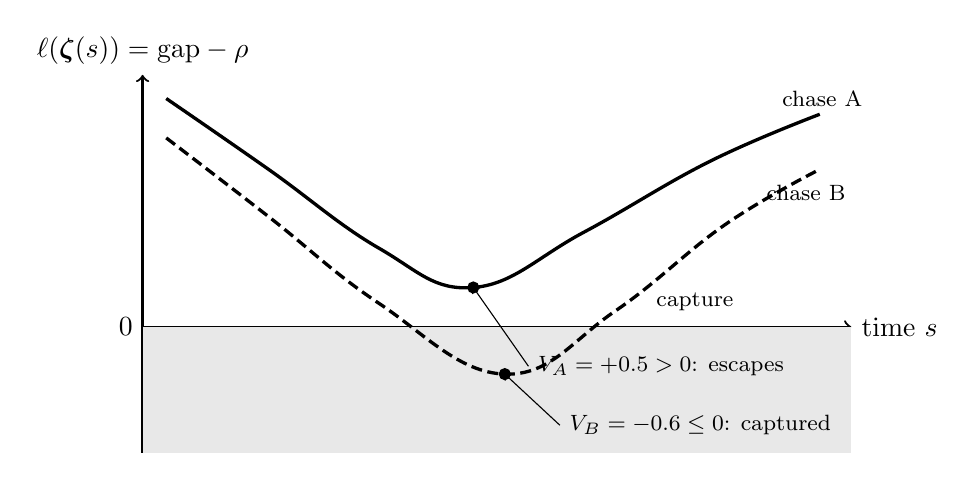
\begin{tikzpicture}[scale=1.0]
% axes
\draw[->,thick] (0,0) -- (9,0) node[right] {time $s$};
\draw[->,thick] (0,-1.6) -- (0,3.2) node[above] {$\ell(\zbf(s))=\text{gap}-\rho$};
% zero (capture threshold) line
\draw[dashed] (0,0) -- (9,0);
\node[left] at (0,0) {$0$};
\node[align=left,anchor=west] at (6.4,0.32) {\footnotesize capture};
\node[align=left,anchor=west] at (6.4,-0.32) {\footnotesize threshold};
% shade capture region
\fill[gray!18] (0,-1.6) rectangle (9,0);
% curve A: not captured (stays above 0), min at 0.5
\draw[very thick] plot[smooth,tension=0.7] coordinates
  {(0.3,2.9) (1.6,2.0) (3.0,1.0) (4.2,0.5) (5.6,1.2) (7.2,2.1) (8.6,2.7)};
\node[anchor=west] at (8.0,2.9) {\footnotesize chase A};
\filldraw (4.2,0.5) circle (2pt);
\draw[<-] (4.2,0.5) -- (4.9,-0.5) node[anchor=west] {\footnotesize $V_A=+0.5>0$: escapes};
% curve B: captured (dips below 0), min at -0.6
\draw[very thick,dash pattern=on 4pt off 2pt] plot[smooth,tension=0.7] coordinates
  {(0.3,2.4) (1.6,1.4) (3.0,0.3) (4.6,-0.6) (6.0,0.2) (7.4,1.3) (8.6,2.0)};
\node[anchor=west] at (7.8,1.7) {\footnotesize chase B};
\filldraw (4.6,-0.6) circle (2pt);
\draw[<-] (4.6,-0.6) -- (5.3,-1.25) node[anchor=west] {\footnotesize $V_B=-0.6\le0$: captured};
\end{tikzpicture}
\caption{The value function is the \emph{lowest point} of the closest-approach curve under the
best chase. For each starting state the pursuer plays optimally; $V$ is the minimum of
$\ell$ over the resulting trajectory. If $V\le0$ (chase B) the trajectory enters the capture set
and the state lies in the backward reachable tube; if $V>0$ (chase A) it does not.}
\label{fig:value}
\end{figure}

\subsection{Formal definition}

For $t\in[-T,0]$, let $\xi^{\ubf_i}_{\zbf,t}(s)$ denote the state at time $s$ of the solution of
\eqref{eq:affine} started at $\xi(t)=\zbf$ under the admissible control signal
$\ubf_i(\cdot):[t,0]\to\Ein$ (measurable), and let $\mathcal{U}$ be the set of such signals. The
value function is
\begin{equation}\label{eq:value}
\boxed{\;V(\zbf,t)=\inf_{\ubf_i(\cdot)\in\mathcal{U}}\ \min_{s\in[t,0]}\ \ell\big(\xi^{\ubf_i}_{\zbf,t}(s)\big)\;}
\qquad\Longrightarrow\qquad
\mathrm{BRT}(t)=\{\zbf:V(\zbf,t)\le0\}.
\end{equation}
The infimum over control expresses the pursuer playing optimally; the minimum over time picks the
instant of closest approach. Two elementary consequences follow directly:
\begin{align}
V(\zbf,t)&\le\ell(\zbf)\quad\text{for all }t\le0
&&\text{(since $s=t$ is in the interval and $\xi(t)=\zbf$),}\label{eq:tube}\\
V(\zbf,0)&=\ell(\zbf) &&\text{(no time left to act).}\label{eq:terminal}
\end{align}

\section{The HJB variational inequality via dynamic programming}

\subsection{Dynamic programming principle}

The value \eqref{eq:value} satisfies, for any small step $\delta>0$, the dynamic programming
principle (DPP)
\begin{equation}\label{eq:dpp}
V(\zbf,t)=\inf_{\ubf_i(\cdot)}\ \min\Big\{\ \min_{s\in[t,t+\delta]}\ell(\xi(s)),\ \
V\big(\xi(t+\delta),\,t+\delta\big)\Big\}.
\end{equation}
In words: the closest approach over $[t,0]$ equals the smaller of the closest approach over the
first sub-interval $[t,t+\delta]$ and the best achievable from wherever the state lands at
$t+\delta$. This is the mathematical statement of ``plan the next instant, then continue
optimally,'' i.e. backward planning.

\subsection{Passing to the differential form}

Assume momentarily that $V$ is smooth near $(\zbf,t)$. Two cases arise in \eqref{eq:dpp}.

\emph{Case 1 (constraint slack, $V<\ell$).} For $\delta$ small the near-term minimum
$\min_{s\in[t,t+\delta]}\ell(\xi(s))$ is not active, so
$V(\zbf,t)=\inf_{\ubf_i}V(\xi(t+\delta),t+\delta)$. A first-order Taylor expansion,
$V(\xi(t+\delta),t+\delta)=V(\zbf,t)+\delta\big(\partial_t V+\inner{\nabla V}{\abf+\Gbf_i\ubf_i}\big)+o(\delta)$,
and cancellation of $V(\zbf,t)$, division by $\delta$, and $\delta\to0$ give
\begin{equation}
0=\partial_t V+\min_{\ubf_i\in\Ein}\inner{\nabla V}{\abf+\Gbf_i\ubf_i}
=\partial_t V+H(\zbf,\nabla V).
\end{equation}

\emph{Case 2 (constraint active, $V=\ell$).} Here the near-term minimum binds and
$\ell(\zbf)-V(\zbf,t)=0$, while the tube inequality \eqref{eq:tube} guarantees
$\ell-V\ge0$ everywhere and $\partial_t V+H\ge0$ in this region.

The two cases combine, exactly, into the single \emph{variational inequality}
\begin{equation}\label{eq:VI}
\boxed{\;\min\Big\{\ \partial_t V(\zbf,t)+H(\zbf,\nabla V),\ \ \ell(\zbf)-V(\zbf,t)\ \Big\}=0\;},
\qquad V(\zbf,0)=\ell(\zbf),
\end{equation}
with $H$ the single-minimisation Hamiltonian \eqref{eq:ham}. Note there is \emph{no} Laplacian
and no artificial-viscosity term in \eqref{eq:VI}: it is a first-order equation.

\section{Viscosity solution: definition, necessity, and uniqueness}

The derivation above assumed $V$ smooth, but $V$ generically has ridges (gradient discontinuities)
wherever two distinct optimal chases tie, and at the moving front of the tube. There the classical
equation is meaningless, and the correct notion of solution is the viscosity solution.

\begin{definition}[Viscosity solution]\label{def:visc}
Writing \eqref{eq:VI} as $F(\zbf,t,V,\partial_tV,\nabla V)=0$ with
$F=\min\{\partial_tV+H,\ \ell-V\}$, a continuous $V$ with $V(\cdot,0)=\ell$ is:
\begin{itemize}[nosep]
\item a \emph{viscosity subsolution} if, for every smooth test function $\varphi$ and every local
maximum $(\zbf_0,t_0)$ of $V-\varphi$, $\;F(\zbf_0,t_0,V,\partial_t\varphi,\nabla\varphi)\ge0$;
\item a \emph{viscosity supersolution} if, for every smooth $\varphi$ and every local minimum of
$V-\varphi$, $\;F(\zbf_0,t_0,V,\partial_t\varphi,\nabla\varphi)\le0$;
\item a \emph{viscosity solution} if it is both.
\end{itemize}
The test function $\varphi$ supplies the gradient at points where $\nabla V$ does not exist; this
is how the ridges are handled without any smoothing.
\end{definition}

\begin{remark}[Two distinct meanings of ``viscosity'']
The \emph{viscosity solution} (Definition~\ref{def:visc}) is the unique correct weak solution and
is unavoidable: it is what ``the backward reachable tube'' means. The \emph{viscosity term}
$\varepsilon\Delta V$ is a numerical device (one of several) for reaching that solution; it is not
part of the definition and need not appear in the equation or the loss. The object is named after
the historical vanishing-viscosity construction $V=\lim_{\varepsilon\to0}V^\varepsilon$, but it can
be reached by methods containing no $\varepsilon$.
\end{remark}

\begin{theorem}[Uniqueness by comparison]
Under a Lipschitz Hamiltonian and the terminal condition \eqref{eq:terminal}, the comparison
principle holds: any viscosity subsolution lies below any viscosity supersolution that dominates it
at $t=0$. Consequently \eqref{eq:VI} has \emph{at most one} viscosity solution, and the value
function \eqref{eq:value} is exactly that solution. Hence the backward reachable tube is
well-defined and unique.
\end{theorem}

\paragraph{Selection example (no viscosity term).} For $|u'(x)|=1$ on $[-1,1]$, $u(\pm1)=0$, the
tent $u(x)=1-|x|$ is the viscosity solution: at $x=0$ its superdifferential is $[-1,1]$ and the
subsolution test $|p|-1\le0$ holds for all $p\in[-1,1]$. The inverted tent $u(x)=|x|-1$ satisfies
$|u'|=1$ wherever differentiable but fails the supersolution test at $p=0$ ($-1\not\ge0$), so it is
rejected. Definition~\ref{def:visc} selects the correct solution and delivers uniqueness using only
one-sided differentials --- with no $\varepsilon$ anywhere.

\section{Physics-informed neural network solution method}

\subsection{Network and terminal condition}

Represent the value function by a sinusoidal-activation network $V_\theta(\zbf,t)$ (sinusoidal
activations represent the value function \emph{and its gradients} markedly better than
$\tanh$/ReLU). The terminal condition \eqref{eq:terminal} is enforced either as a soft loss term
plus terminal pre-training, or with an exact-boundary-condition ansatz of the form
\begin{equation}
V_\theta(\zbf,t)=\ell(\zbf)+t\cdot c_{\max}\cdot\tfrac{1}{2}\big(\tanh(N_\theta(\zbf,t))+1\big),
\end{equation}
where $N_\theta$ is the network and $c_{\max}>0$ bounds the terminal rate of change. For $t\le0$
the correction is $\le0$, so $V_\theta\le\ell$, consistent with the tube property \eqref{eq:tube}.
(The previous draft used $\tfrac12(\tanh-1)$, which forces $V_\theta\ge\ell$ and collapses the tube;
this is corrected here.)

\subsection{Loss and curriculum}

Training minimises the residual of the variational inequality \eqref{eq:VI}, with the costate
$\pbf=\nabla_{\zbf}V_\theta$ obtained by automatic differentiation:
\begin{equation}\label{eq:loss}
\mathcal{L}(\theta)=
\underbrace{\mathbb{E}_{\zbf}\big[\|V_\theta(\zbf,0)-\ell(\zbf)\|\big]}_{\text{terminal condition}}
+\lambda\,
\underbrace{\mathbb{E}_{\zbf,t}\Big[\big\|\min\{\partial_tV_\theta+H(\zbf,\nabla V_\theta),\ \ell(\zbf)-V_\theta\}\big\|\Big]}_{\text{variational-inequality residual}} .
\end{equation}
The terminal condition is propagated backward in time by \emph{curriculum learning}: $t$ is swept
slowly from $0$ toward $-T$ as training progresses. This causal sweep is the mechanism that steers
the network onto the viscosity solution; no artificial-viscosity term is required.

\subsection{Optional vanishing-viscosity stabiliser}

If early training is unstable, a vanishing-viscosity term may be added \emph{to the residual only},
\begin{equation}
\partial_tV_\theta+H(\zbf,\nabla V_\theta)-\varepsilon_{\mathrm{visc}}\,\Delta_{\zbf}V_\theta,
\end{equation}
with the full nine-dimensional Laplacian $\Delta_{\zbf}$ and $\varepsilon_{\mathrm{visc}}$ annealed
to zero on a schedule. It must vanish by the end of training, because the target is the
$\varepsilon_{\mathrm{visc}}=0$ solution. A restricted Laplacian in only the position coordinates is
\emph{not} a valid selector and is not used.

\section{Verification protocol}

No neural approximation is self-certifying, so the computed tube must be verified:
\begin{enumerate}[nosep]
\item \textbf{Convergent-solver benchmark.} Compare $\{V_\theta\le0\}$ against a Level Set Toolbox
solution (essentially-non-oscillatory spatial differences, total-variation-diminishing time
stepping) on a reduced-dimension model; agreement on the tube \emph{boundary} and the ridge
locations is the relevant test, not the smooth interior.
\item \textbf{Closed-loop rollout.} Synthesise the pursuer control $\ubf_i^\star(\nabla V_\theta)$,
simulate against the APF evader, and confirm that the realised closest approach matches $V_\theta$.
\item \textbf{Self-consistency.} Check the dynamic programming principle \eqref{eq:dpp} on sampled
states and confirm monotone growth of the tube in reverse time.
\end{enumerate}

\section{Summary}

\begin{center}
\begin{tabular}{@{}ll@{}}
\toprule
\textbf{Element} & \textbf{Specification}\\
\midrule
State & $\zbf=(X,Y,\psi_{\mathrm{rel}},u_e,v_e,u_i,v_i,r_e,r_i)^\top\in\R^9$ (pursuer body frame; $\psi_{\mathrm{rel}}$ encoded as $\cos/\sin$ to the network)\\
Dynamics & $\dot{\zbf}=\abf(\zbf)+\Gbf_i\ubf_i$ (control-affine, pursuer only)\\
Evader & fixed repulsive APF, folded into $\abf$\\
Actuator set & inscribed ellipse $\Ein$, offset centre $\ubf_0=(F_{\max},0)$, Eq.~\eqref{eq:Ein}\\
Equation type & HJB variational inequality (single minimisation)\\
Terminal cost & $\ell(\zbf)=\sqrt{X^2+Y^2}-\rho$\\
Hamiltonian & $H=\pbf^\top\abf+\tfrac{F_{\max}}{M_{11}^i}p_{u_i}-\sqrt{\cdots}$, Eq.~\eqref{eq:ham}\\
Value function & $V=\inf_{\ubf_i}\min_{s\in[t,0]}\ell(\xi(s))$, Eq.~\eqref{eq:value}\\
Solution concept & unique viscosity solution (no $\varepsilon$ in the definition)\\
Solver & sinusoidal PINN, corrected terminal ansatz, backward-time curriculum\\
Verification & Level Set Toolbox benchmark + closed-loop rollout\\
\bottomrule
\end{tabular}
\end{center}

\paragraph{Key references.} R. Isaacs, \emph{Differential Games} (1965); M. G. Crandall and
P.-L. Lions, ``Viscosity solutions of Hamilton--Jacobi equations,'' \emph{Trans. AMS} (1983);
M. Bardi and I. Capuzzo-Dolcetta, \emph{Optimal Control and Viscosity Solutions of
Hamilton--Jacobi--Bellman Equations} (1997); A. B. Kurzhanski and P. Varaiya, ``Ellipsoidal
techniques for reachability analysis'' (2000, 2002); S. Bansal, M. Chen, S. Herbert, C. Tomlin,
``Hamilton--Jacobi Reachability: A Brief Overview and Recent Advances,'' CDC (2017); S. Bansal and
C. Tomlin, ``DeepReach,'' ICRA (2021); T. A. Johansen and T. I. Fossen, ``Control allocation --- A
survey,'' \emph{Automatica} (2013).

\end{document}
